% !TeX root = ../main.tex

\chapter{相关技术介绍}

\section{卷积神经网络}

深度学习中一种常见的网络架构就是卷积神经网络,其是在生物自然视觉认知机制的启发下发展而来。1959年,Hubel  Wiesel  发现了视觉系统的信息处理,可视皮层是分级的。比如人眼在观察一个物体时,从瞳孔摄入信息开始,先做初步处理:大脑皮层的相应功能部分对物体的边缘和方向进行识别,然后再进行抽象:大脑判定,眼前的物体的形状等信息,最后进一步抽象处理,大脑进一步分析判定该物体的类别。

现代的CNN结构是由20世纪 90年代,LeCun等人发表论文确立的,后来学者又对其进行完善。他们当时设计了一种叫做LeNet-5的可以对手写数字做分类的多层的神经网络,见\cite{LeNet}。

CNN能够从输入的原始像素中,识别空间局部的特征。然而当时既缺乏大量的训练数据又缺乏算力强的计算机,这导致了LeNet-5对于复杂问题的处理效果很不理想。为了解决难以训练深度卷积神经网络的困难,很多专家学者先后提出了很多方法。其中,最著名的是Krizhevsky et al.提出的AlexNet\cite{AlexNet},其在图像识别任务上取得了重大突破,同时也让卷积神经网络的研究进入了一个新的高度。在那之后,研究人员又提出了一系列新的改进方法,其中最著名的要数ZFNet\cite{ZFNet}, VGGNet\cite{VGG}, GoogleNet\cite{Google}和ResNet\cite{Resnet}这四种。从结构看,CNN发展的一个方向就是层数变得更多,ILSVRC 2015冠军 ResNet\cite{Resnet}是 AlexNet\cite{AlexNet}的20多倍,是 VGGNet\cite{VGG}的8倍多。虽然通过增加深度,同时使用非线性激活函数ReLu与Dropout的方法,利用增加的非线性网络能够得出与目标函数的近似结构。但是,这样做也使得网络整体变得更复杂,并且很难去优化。

卷积神经网络一般由两层组成:特征提取层与特征映射层。

在特征提取层中,为了能够提取局部特征,每个神经元的输入与前一层的输出相连。而且它与其它特征间的关系在局部特征被提取后也会被确定下来;

在特征映射层中,若干个特征映射组成网络的计算层,其中每个特征映射是一个平面,并且上面所有神经元的权值均相等。特征映射结构采用非线性的sigmoid激活函数。特征映射层上的神经元的权值共享机制,也减少了网络中参数的个数。这种每个卷积层都跟着一个计算层的提取结构减小了特征分辨率。



\subsection{卷积神经网络的基本结构}

卷积层、池化层、全连接层、激活层与回归层构成卷积神经网络的主体结构。
它的输入通常先经过卷积层与激活层,然后再通过池化层输出作为其中的一步结果,这种结构堆叠若干次后(每堆叠一次即增加一层深度),再接上全连接层、回归层运算得出最终的输出结果。这样便构成了卷积神经网络的完整网络结构,上述步骤的简化模型如图\ref{cnn}所示。

\begin{figure}
	\center
	{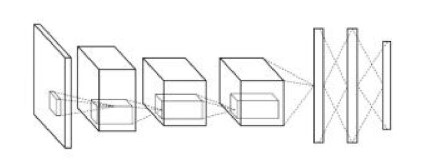
\includegraphics{cnn.jpg}}
	\caption{卷积神经网络模型}
	\label{cnn}
\end{figure}

卷积神经网络的输入内容通常为图像(由像素矩阵构成的位图)或其他多维的数据,输出为如分类标签或者目标位置的检测目标值。接下来对各层的作用进行具体说明。

卷积层((Convolutions layer):用来学习特征(对于接受输入的数据)。卷积层由很多的卷积核(convolutional kernel)组成,不同的卷积核用来计算不同尺度的特征图(feature map)。
卷积层的本质就是许多不同尺度的滤波器。
每个滤波器由三维的矩阵构成。其中前两维是滤波器的尺寸(即卷积核的大小),第三维为其深度,它是由输入的特征图的深度决定其值,其中初始输入图像的深度为颜色通道数(位图为RGB-3个通道)。并且在使用同一个卷积核的情况下,特征图可以共享该卷积核的权值,这样就能减少很多的网络参数,使运算更为简化。

激活层(activation layer):由于卷积操作过程是线性的,而实际图像的特征通常都是非线性的。因此,想要提高网络结构的非线性的表达能力就需要在卷积神经网络中加入激活函数。引入了非线性后,卷积神经网络便能够匹配期望的目标函数。深度学习中通常使用的激活函数有sigmoid、tanh、ReLU等。

池化层(Pooling layer):用来降低卷积层输出的特征向量的维度。这样不仅可以减少神经网络参数的数量,而且还能够改善运算结果,使网络结构能过正常工作,同时还可以让网络不易出现过拟合现象。池化层的本质是二维滤波器,常见的池化层的操作有平均池化和最大化池化等。

网络可以通过堆叠卷积层与池化层从而获得图像的更多抽象特征。

全连接层(Full connected layer):卷积层和池化层堆叠之后,就能够形成一层或多层全连接层,能够实现整合能力,起到分类器的作用。全连接层能够从前面卷积池化层学到的特征图映射到与之对应的样本空间。全连接层的每一个节点都和上一层的所有节点相连,获得一维向量的输出。全连接层常用sigmoid/tanh非线性函数。

\subsection{卷积神经网络的训练过程}
卷积神经网络的训练过程主要包括前向传播和误差反向传播,它实际上就是让网络各层的神经元节点更新它们的权值,以得到较好的模型。

\subsubsection{前向传播}

前向传播是指卷积神经网络将提取到的特征在模型中的以正向的次序进行传递。特征依次按照顺序经过卷积神经网络的各层结构。
这个过程中包含了局部感知、权重共享和下采样这三项主要内容。

\paragraph{局部感知}使用小于输入特征图尺寸的卷积核对其进行扫描,然后在每个位置都进行卷积运算是局部感知的主要操作。由于在图像中,局部联系通常比全局联系更密切,并且符合人感知视觉从局部到全局的特点,因此只感受局部信息而不是全局的信息就可以得出有效的特征。
故在这种方式下,层中的每个节点只需要与图像上某个局部的像素点相连,这样做也减少了训练时的权值参数,提高了计算性能。

\paragraph{权重共享}权重共享指的是对同一张图像均使用同一个卷积核进行单次扫描。由于在同一张图像中,每一个局部的统计特性具有共性,故共享卷积核的操作能够减少权值参数,便于计算。在每个卷积核遍历接受输入的特征图时,每个位置处均是共享一组权重的,因此不需要去单独学习图像中各个位置的权重。

\paragraph{下采样}它本质上就是池化过程。由于经过池化过程能够缩小图像的规模(卷积神经网络中,池化操作并不会损失重要的局部信息),因此可以减少计算量,并且减少了训练参数,不易出现过拟合现象。

以上三种方法每步都能减少计算步骤,从而组合来使用不但可以极大地减少各层节点之间的连接数量,而且还能够有效的提升网络的计算处理性能。

\subsubsection{反向传播}

反向传播是指卷积神经网络输出的特征和标准特征($Ground$ $Truth$)之间存在误差,我们可以利用这些误差信息根据一些特定的计算方法在模型中按照反向的次序调整各层神经元的权值,从而实现对网络整体的各参数进行调整。常见的损失函数有交叉熵、均方差、对数似然等。

\subsubsection{整体过程}

如图\ref{cnn-process}所示,一幅图像通过卷积神经网络的过程就是:

\paragraph{前向传播过程}

首先对其进行卷积的操作,输出特征图。
得到特征图后,对特征图进行池化操作,然后使用激活函数处理。
反复重复这个过程多次之后,再通过全连接层与目标结果建立映射关系,得出训练结果。

\paragraph{反向传播过程}

在反向传播过程中,网络需要对训练结果与真实值($Ground$ $Truth$)使用某种损失函数进行误差计算,然后根据运算结果与网络实际结构综合来更新各层神经元的权值。

\begin{figure}
	\center
	{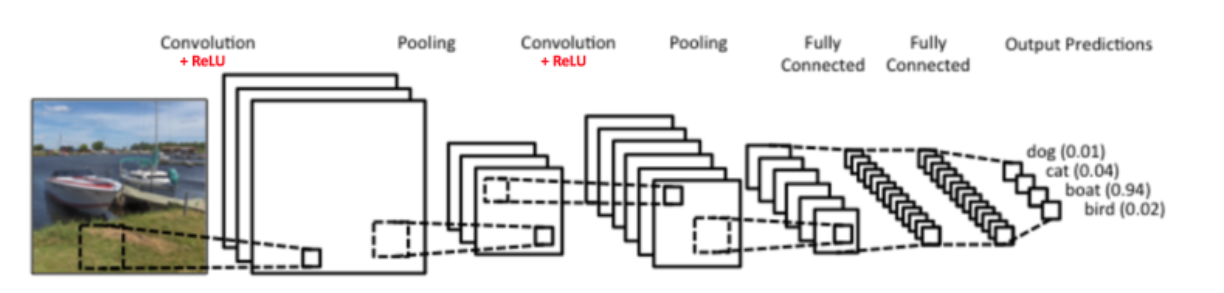
\includegraphics[width=12cm,height=3cm]{cnn-process.png}}
	\caption{卷积神经网络训练过程}
	\label{cnn-process}
\end{figure}

\subsection{深度网络的退化问题}

网络的深度对模型的总体性能有着重要作用。理论上说,网络层数增加后,网络可以对更加复杂的特征进行提取,所以应该可以取得更好的结果。但是更深的网络结构的性能不一定会更好。实验结果发现增加网络深度时会出现退化问题:当网络层数增加时,网络训练结果的准确度会出现饱和,深度过大时甚至出现准确度下降的现象。这个现象可以在图\ref{WangLuoTuiHua}中直观看出来:56层的网络比20层得网络效果还要差。因为56层网络的训练误差同样高,所以这也不会是过拟合得问题。由于深层网络很可能会出现梯度消失或者梯度爆炸的问题,这就使得深度学习模型得训练过程会很艰难。虽然现在已经存在一些如BatchNorm的技术手段来缓解这个问题,但是效果仍然不是很理想,仍需要一个更加优秀的网络模型来解决这一问题。

\begin{figure}
	\center
	{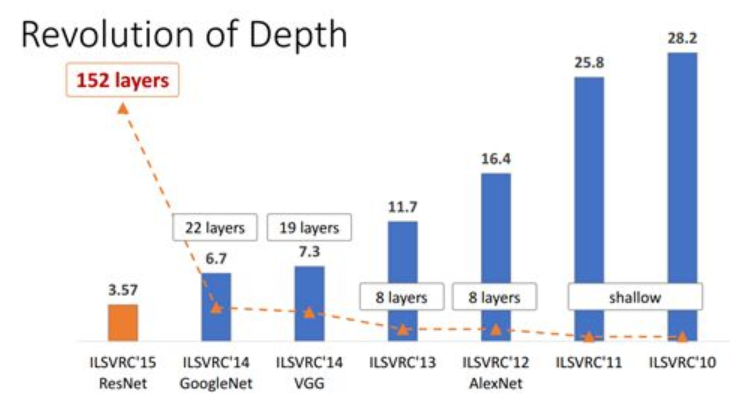
\includegraphics[width=10cm,height=5.5cm]{WangLuoTuiHua.png}}
	\caption{神经网络的退化问题}
	\label{WangLuoTuiHua}
\end{figure}

\subsection{残差学习}

最近几年深度学习发展迅速,出现了很多优秀的CNN网络结构,例如AlexNet、VGG、GoogLeNet、ResNet等。

VGG\cite{VGG}是Oxford的Visual Geometry Group的组提出的。该网络说明了网络深度的增加在一定程度上会影响网络的表现性能。VGG\cite{VGG}有两种结构,分别是VGG16和VGG19,二者只是在网络深度上不同,并没有本质上的区别。VGG16相对于AlexNet\cite{AlexNet}的其中一个改进是将AlexNet中的较大卷积核(11$\times$11,7$\times$7,5$\times$5)用连续的几个3x3的卷积核来代替。由于多层非线性层可以增加网络深度来保证学习更复杂的模式,因此采用堆积的小卷积核在给定的感受野的情况下优于采用大的卷积核,提升了网络的深度,在一定程度上提升了神经网络的效果。并且其参数较AlexNet更少,计算开销更小。但是VGG仍然耗费了很多的计算资源,仍使用了较多的参数,导致内存占用较大,整体效果不是特别理想。

ResNet\cite{Resnet}是微软团队开发的网络。它的特征在于具有比以前的网络更深的结构。虽然加深层对于提升性能很重要。但是,可能会出现上面提到的退化问题,导致最终性能不佳。为了解决这样的问题,ResNet提出了一种“快捷结构”。使用了这种快捷结构后,随着层数的加深网络在一定限度内就可以而不断提升性能了。

快捷结构,将输入的x加到输出中,跳过了输入数据的卷积层。
如图\ref{ResnetStructure}所示,在连续的卷积层中,输入的x一方面进入卷积池化层进行运算,另一方面存储下来直接加到前面运算的结果上。即通过里的快捷结构,使原来的输出由F(x)变为了F(x)+x。由于采用这种结构后,反向传播时的信号可以无衰减地进行传递,防止了由于深度增加而引起的梯度消失或爆炸问题。因此,即便是加深层数,Renet网络也能高效地学习。

\begin{figure}
	\center
	{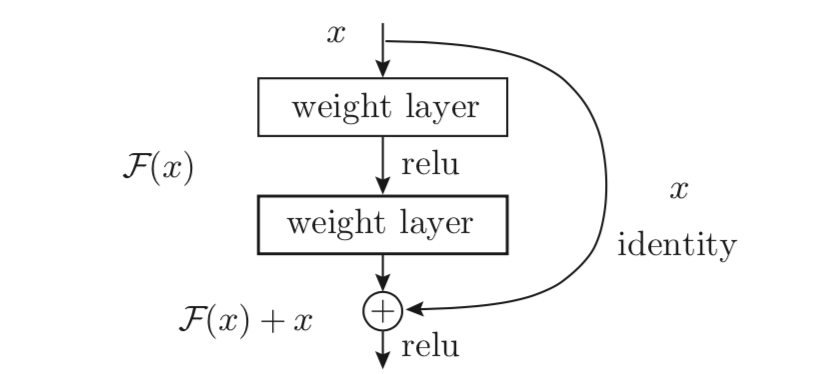
\includegraphics[width=12cm,height=6cm]{ResnetStructure.png}}
	\caption{Resnet中快捷结构示意图}
	\label{ResnetStructure}
\end{figure}

ResNet以VGG网络为基础,引入快捷结构以加深层并且能够避免退化问题,其结构如图\ref{ResnetDemo}所示。

\begin{figure}
	%\center
	{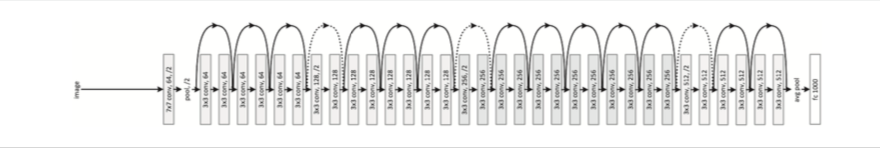
\includegraphics[width=13cm,height=3cm]{ResnetDemo.png}}
	\caption{Resnet模型结构示意图}
	\label{ResnetDemo}
\end{figure}

ResNet使用跳跃式的连接方法来加深层(以两个卷积层为间隔)。实验结果显示,即使层数以及达到了150以上,检测结果的准确性也会持续提高。在ILSVRC大赛中,ResNet的Top5错误识别率为3.5\%,如此优秀的表现真是令人称奇。

Resnet在精度、速度上都比VGG表现好很多,因此,现阶段大部分模型都选择将Resnet作为主干网络进行训练。

\section{目标检测器}
通常,目标检测器可以分为两类:一阶段目标检测器和两阶段目标检测器。两阶段目标检测器,如Mask R-CNN\cite{MRCNN}、Fast R-CNN\cite{FRCNN}、Faster R-CNN\cite{Faster}是提取感兴趣的区域进行检测和识别,由于其包含一个用于区域建议的预处理步骤,使得整体流程是两阶段式的。由于处理的步骤多以及阶段耦合的原因,两阶段的目标检测器效率很低,不能够满足实时任务的要求。一阶段目标检测器,如YOLO\cite{YOLO}、DES\cite{DES}和SSD\cite{SSD}等直接训练产生出物体的置信度和坐标位置,将所有计算(划分候选框与识别)封装在一个网络中,从而在根本上很大程度的提高了检测速度。一阶段检测器分为基于候选框的和无候选框的。候选框是在神经网络初始化时预先生成的不同尺寸和比例的物体候选框。一阶段基于候选框的检测器直接预测候选框的偏移和类别。经典网络有基于SSD的检测器,如DSSD\cite{DSSD}、FSSD\cite{FSSD}。一阶段基于无候选框的直接预测物体的坐标和类别,比如Cornernet\cite{CornerNet}预测了几个关键点,然后将这些点分成对,即对象左上角和右下角的坐标。但是由于其缺乏候选框机制而导致预测不稳定,这就需要使用更大的输入图像输入和更复杂的模型来训练。同时,其还需要额外的操作优化算法,否则网络会产生大量背景或错误的关键点,从而降低检测精度。

\subsection{两阶段目标检测器}
两阶段目标检测器因其有着一个用于区域建议的预处理步骤,因此也被称为基于区域(Region-based)的方法,R-CNN系列模型是这一类型的代表。

R-CNN\cite{RCNN}将检测划分为两阶段,第一阶段是基于图片训练提出一系列可能包含物体的区域(Region Proposal),原论文中使用的是Selective Search算法;第二阶段是在提出的这些建议区域上运行分类网络(使用当时效果最好的AlexNet\cite{AlexNet}),回归得到每个区域内物体的类别。

文章Fast R-CNN\cite{FRCNN}指出R-CNN耗时的原因之一是其卷积神经网络是在每一个提议区域上单独进行的,并没有共享计算,导致消耗了大量的计算资源。Fast R-CNN在基础网络把图片运行完成后,才传入R-CNN子网络。这样共享了大部分计算,因此其执行效率可以高一些。

Faster R-CNN\cite{FRCNN}在两阶段的目标检测器中有着重要的地位,其将原来的Selective Search算法替换为RPN网络,通过这样的处理可以使得检测任务以很快的速度完成。它是在Fast R-CNN基础上加了RPN网络,去除冗余运算、共享卷积计算的特性使得RPN网络的整体计算量非常小,故Faster R-CNN能够以较高的速度运行,并且在精度方面也能够达到最佳。Faster R-CNN的突出贡献是提出Regional Proposal Networks,替代之前的算法。

RPN网络将区域提议这一任务转化为二分类问题,即其中是否包含物体。
它第一步是在一个滑动窗口上生成不同大小和宽高比的候选框,取定IoU的阈值,按Ground Truth标定这些候选框的正负。即传入RPN网络的样本数据被整理为候选框的(坐标)和每个候选框是否有物体(0,1二分类)。RPN网络对每个样输出一个置信度和四个坐标值信息。置信度表示这个候选框内部包含有有物体中心点的概率,四个坐标值(中心点x,y与宽w高h)用于定位物体的位置。RPN网络训练的损失函数为是否包含物体的二分类值与坐标差值的损失的加权统一。

Faster R-CNN的突出之处在于其用了RPN网络来代替传统的区域提议的方法。使用不同大小和宽高比的候选框的机制也在后面提出的一些模型中被采用(YOLO\cite{YOLO}等)。Faster R-CNN确定了"RPN+RCNN"的模式,奠定了两阶段目标检测的基本结构。

\subsection{一阶段目标检测器}
一阶段目标检测器运行和检测速度非常快,虽然在准确性上比两阶段目标检测器要差一些,但是随着近几年对于相应算法的优化与发展,两种检测器在识别准确性上的差别正在逐渐缩小;因此一阶段目标检测器凭借着其速度优势获得了目标检测中的重要地位。
由于一阶段模型直接从图片获得预测的结果,没有中间的区域提议过程,因此也被称为Region-Free的方法。目前主要的一阶段目标检测算法分为YOLO\cite{YOLO}系列与SSD\cite{SSD}系列。

\subsubsection{YOLO}

如图\ref{YOLO}所示,首先,YOLO\cite{YOLO}将一张输入图片分成$S\times S$格。如果Ground Truth框的中心落在某格上,则该格负责预测这个目标。每格会预测$n$个候选框以及$n$个置信度。该置信度得分表征出的是该格内包含物体的概率有多大以及这个检测出来的预测框与实际的框之间IOU的大小。因此,如果这个格子上面没有物体,则该位置处的得分为0;如果该格上包含有物体的中心,那么其得分应该等于IOU。所以对于每个候选框而言,都会预测5个值,分别是置信度与中心点的横纵坐标,候选框的宽高。

对于划分的每个格子而言,除了预测$n$个候选框的信息以及其置信度的大小外,它同时还会预测$c$个类别的条件概率。VOC2007、2012数据集中包含了20个类,所以它就会预测$n$=21个类别(多的一个类是背景)的概率。其中这个概率是在确定候选框中存在实际目标的情况下,该目标为第$i$类的条件概率。每个候选框会共享这样的概率,与$n$个候选框无关。
不难看出,每格中物体的具体类别的置信度不但反映出这个类别出现在这里出现的概率,而且同时也反映出了该预测框与实际框($Ground$ $Truth$)之间的相似度有多大,即检测结果是否符合标准。

\begin{figure}
	\center
	{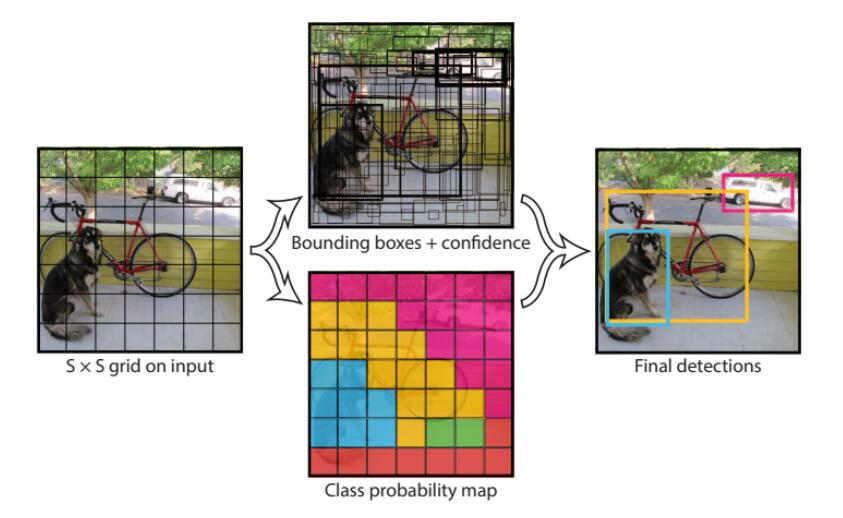
\includegraphics[width=16.86cm,height=10.36cm]{YOLO.jpg}}
	\caption{YOLO预测}
	\label{YOLO}
\end{figure}

如图\ref{YOLOStructure}所示,如果单纯从网络结构考虑,YOLO和普通的用卷积神经网络进行分类的网络基本没有什么区别,因为去掉候选框处理的这个步骤后,YOLO的结构非常简单,就是单纯的卷积、池化最后加了两层全连接层。它们最大的差异是YOLO最后输出的地方采用的是线性函数作为激活函数,因为它不仅仅是预测某类的概率,还需要预测Bounding Box的位置。所以整体上来说,YOLO的整个结构就是通过神经网络的变换把输入的图片映射成一个输出的向量。


\begin{figure}
	\center
	{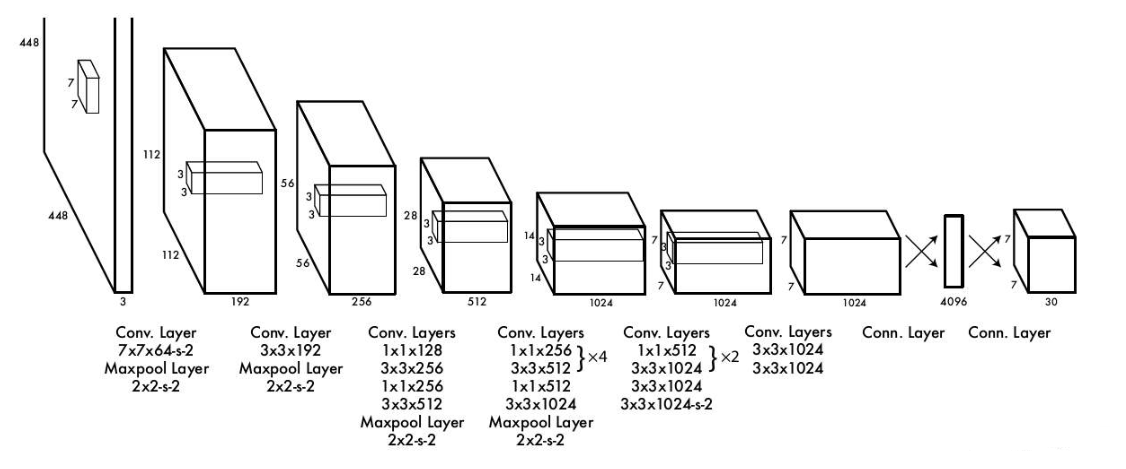
\includegraphics[width=16cm,height=7cm]{YOLOStructure.png}}
	\caption{YOLO网络结构}
	\label{YOLOStructure}
\end{figure}

\subsubsection{SSD}

SSD\cite{SSD}的网络结构如图\ref{SSDStructure}所示,其使用了($38\times 38$),($19\times 19$),($10\times 10$),($5\times 5$),($3\times 3$),($1\times 1$)6个不同尺度的特征图来预测分类。这6个特征层会分别经过$3\times 3$的卷积后转化为包含置信度和坐标偏差的通道。由于SSD使用了更多的特征层,因此与YOLO\cite{YOLO}相比,它更适合检测拥有多种不同尺度目标的图像。

同时,在这6种不同尺寸的金字塔结构输出的特征图中,SSD还使用了不同大小、不同宽高比的候选框。每层特征图使用不同于其他层的大小的候选框,并且根据具体的特征图尺度设置4种或者6种的宽高比来框出检测物体。之后的很多基于SSD的改进拓展网络都采取这种候选框方式。

与之前的网络相比,SSD并没有使用所有的负样本,而是对这些匹配上背景的样本处理得到的由置信度损失按照降序排列,把其中损失较大的样本记作难例(hard negative),当作该模型需要重点学习的对象。把其中损失结果最大的前N个样本当作负样本(其中正样本与负样本的比例控制需要在1:3左右)。而对于那些没有被选上的样本,SSD把其标签设置为-1,即它以后不再参与训练。

论文说明数据增强处理能够明显提升网络的性能。即采用数据增强的步骤,能够彰显样本之间的多样性与差异性,从而极大地提升了模型的泛化能力。SSD的高准确率同时也得益于空洞卷积操作。通过空洞卷积,网络能在较少的参数情况下有着较大的感受野,即能使网络能感知到更多的东西。

\begin{figure}
	\center
	{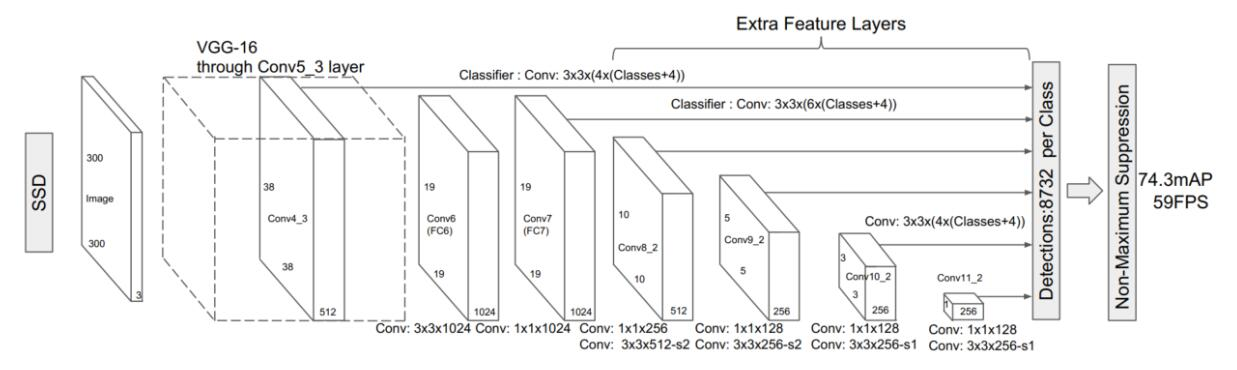
\includegraphics[width=16cm,height=4.7cm]{SSDStructure.jpg}}
	\caption{SSD网络结构}
	\label{SSDStructure}
\end{figure}

SSD奠定了一阶段目标检测的重要模式,其能够在比两阶段目标检测器速度快了近一个量级的情况下维持了较高的准确性。后续大部分的一阶段目标检测器基本是基于对SSD的改进展开研究的。

\section{注意力机制}

注意力模型最初被用于自然语言处理,现在也成为深度学习领域的一个重要模型。注意力机制人工智能领域已成为神经网络结构的重要组成部分,并在自然语言处理、语音识别和计算机视觉等领域有着广泛的应用。

注意力机制仿照了人观察物体的方式。一般而言,当人在看一张图片的时候,除了从整体把握一幅图片的特点之外,通常会对图片的某个局部位置感兴趣,进而注意力集中在相关区域上。例如人像照中人脸的位置,宣传图片中商品的具体位置等。
在翻译一段话的时候,人们通常是从句子的整体内容入手,在阅读句子的过程中,除了需要关注其中出现的词语本身的含义,还要考虑与词语有前后关系的信息以及该词语的上下文信息。在自然语言处理学科中,如果需要对情感进行分类,那么在其中的某个句子中,一定会涉及到一些能够传达出情感的词语。处在该句子里面的其他不相关词语,则是情感词语的上下文。它们并不是对语言表达没有用,而是其对于语义表达的能力远没有那些能够直接表达情感的关键词大。因此,注意力机制是把注意力集中放在重要的信息上,而忽略其他次要的因素。其中重要程度的判断取决于应用场景。%注意力根据应用场景的不同被划分为空间注意力和时间注意力,其中空间注意力用于图像处理,时间注意力用于自然语言处理。

注意力机制的处理结果通常都是以概率张量或者概率图的形式表示。从原理上来说,主要分为空间注意力模型,通道注意力模型,空间和通道混合注意力模型三种。

空间注意力模型:图像中所有的区域对于检测任务的贡献不相同,与任务相关的区域是检测的重点,是需要突出关心的。空间注意力模型就是寻找图像、网络中最重要的部分进行处理。由于我们在大部分情况下所感兴趣的内容只是输入图像中的一个小区域,因此空间注意力的本质就是完成对目标的定位。比如Google DeepMind提出的STN网络(Spatial Transformer Network)\cite{STN}。它通过学习输入的局部重要信息,分析完成适合任务的预处理操作,这用到的是一种基于空间的注意力模型。

通道注意力机制:卷积神经网络的输入是一个二维图像,其中的一个维度是图像的尺度,即宽w高h,另一个维度就是通道数。因此基于通道的注意力机制也是很常用的。通道注意力机制的本质,在于构建了各个特征之间的重要性关系,对不同的任务可以根据输入的区别进行特征分配,处理起来简单有效。例如SENet(Sequeeze and Excitation Net)\cite{SENet}是2017届ImageNet分类比赛的冠军网络,其本质上是一个基于通道的注意力模型,它通过联系各个通道的相关程度,并对不同的任务增强或者抑制不同的通道。

空间和通道注意力机制的融合:CBAM(Convolutional Block Attention Module)\cite{CBAM}是空间和通道注意力机制融合的代表性网络,其结构如图\ref{CBAMStructure}所示,可以看出一个CBAM模块包括两个子模块,其分别进行通道上和空间上的注意力计算,见图\ref{CBAMTwoAtt}。\\

\begin{figure}
	\center
	{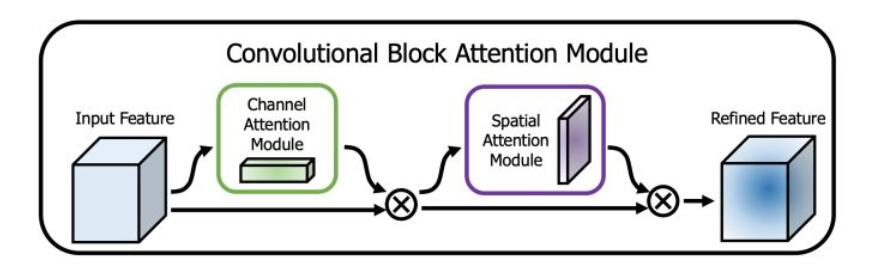
\includegraphics[width=12cm,height=4cm]{CBAMStructure.jpg}}
	\caption{CBAM结构}
	\label{CBAMStructure}
\end{figure}

\begin{figure}
	\center
	{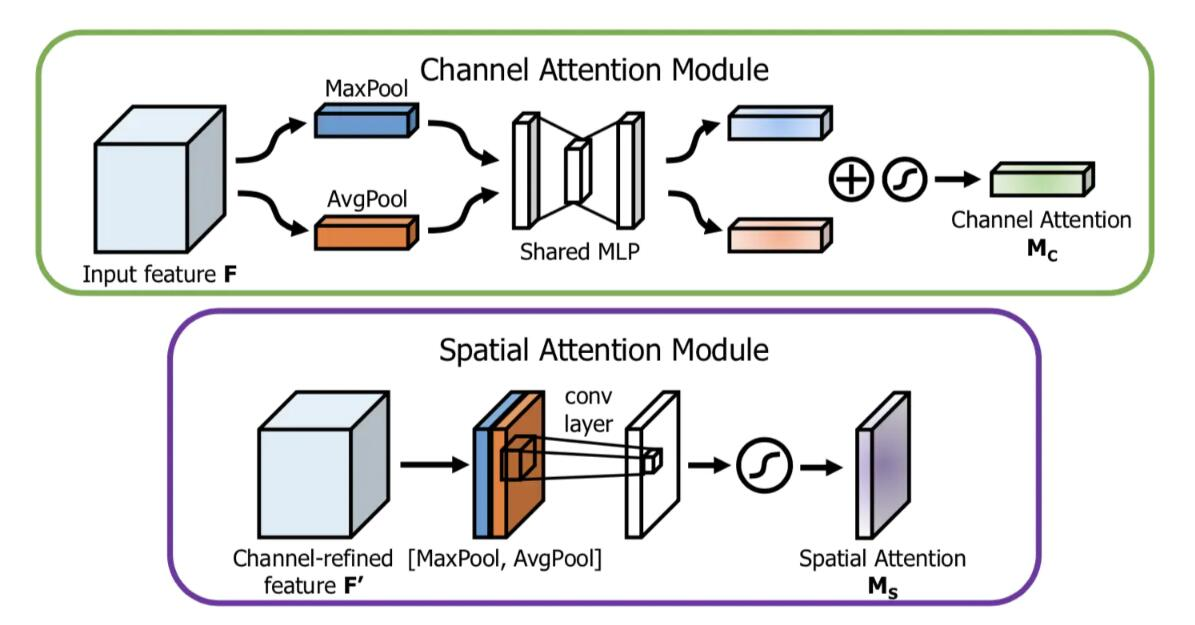
\includegraphics[width=11.95cm,height=6.25cm]{CBAMTwoAtt.jpg}}
	\caption{CBAM空间、通道注意力模型}
	\label{CBAMTwoAtt}
\end{figure}

实验证明,在小模型上添加CBAM模块也能带来较稳定的性能提升,而且这样处理只会增加一点少量的计算,并不会在执行效率上产生显著影响。这个实验结论还说明,模型越大模型的表达能力会更强,性能上也会高一些。虽然小模型在性能上要低一些,但是添加CBAM后同样能看到结果的稳定性能提升。因此这个方法处理效果十分可观。

相比于基准的模型,在添加了CBAM之后,在GRAD-CAM\cite{GCAM}的可视化下,该模型能够实现更加关注目标本身。其执行效果如图\ref{CBAMRes}所示。

\begin{figure}
	\center
	{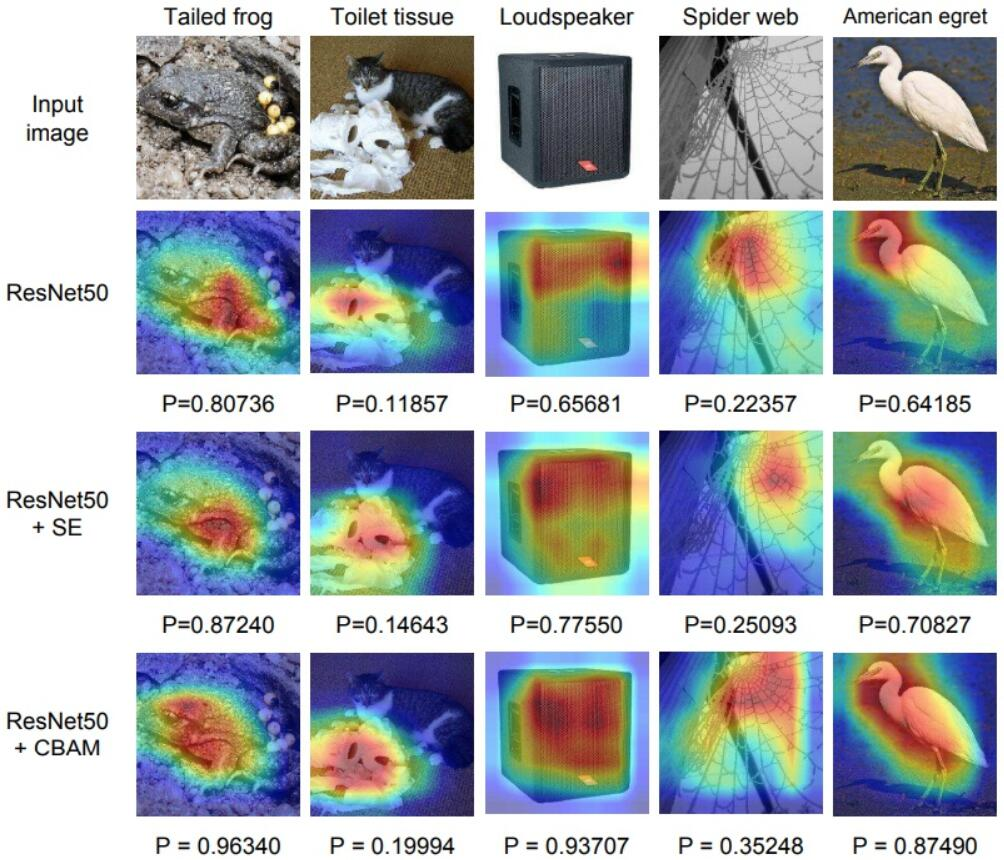
\includegraphics[width=9.75cm,height=8.125cm]{CBAMRes.jpg}}
	\caption{添加CBAM的注意力热力图}
	\label{CBAMRes}
\end{figure}


对于输入图像,注意力图经过运算突出显示了不同尺度大小的有用区域,如图\ref{AttVis}为PASCAL VOC2007数据集中注意力的可视化热力图。注意力图是图片上的每个位置空间特征的加权之和,因此,与特征相关的区域会被突显,不相关区域(如背景)会被抑制。这样做有助于模型关注实际目标,从而提高了检测效率与准确性。

\begin{figure}
	\center
	{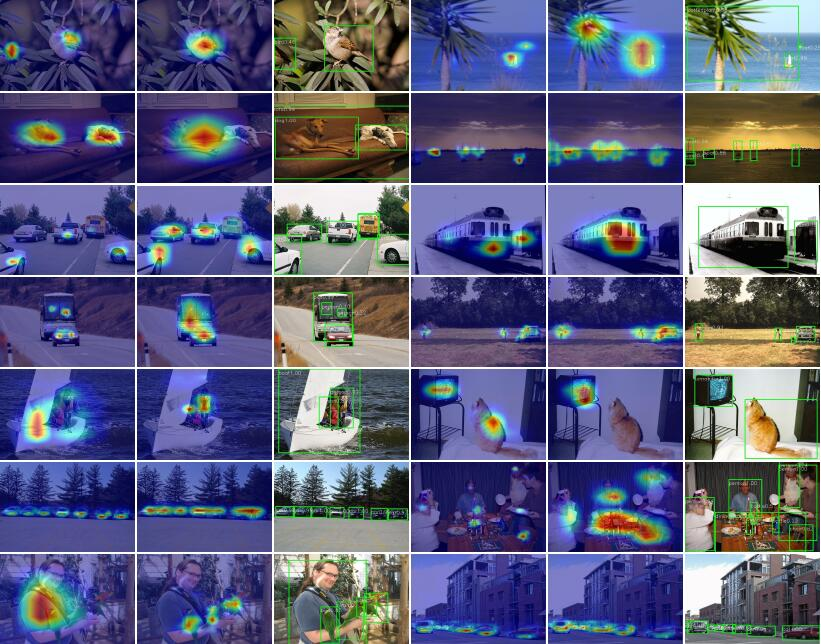
\includegraphics[width=10.673cm,height=8.372cm]{AttVis.jpg}}
	\caption{VOC2007数据集注意力热力图}
	\label{AttVis}
\end{figure}

